% ************ Chapter 3 ************
%\renewcommand{\chaptername}{Chapter}
\chapter{Análise de Valor}
\label{cap:3}
%\emph{Este capitulo incide em apresentar de que forma as diferentes alternativas criam valor para o público alvo, e desta forma tirar conclusões sobre qual alternativa deve ser aprofundada}

Aplicando o modelo de Peter A. Koen, \emph{New Concept Development}, é possível mapear uma oportunidade para um conceito, seguindo todos elementos chave do modelo e percebendo assim
se esta oportunidade representa ou não valor para a organização.

\subsection{Identificação da Oportunidade}
Neste contexto, a oportunidade surge no sentido de prevenir o acontecimento de escândalos como o conhecido Cambridge Analytica e outros "leaks" \cite{cambridge_analytica} de informação que acontecem a um ritmo cada vez superior numa web baseada num paradigma que parece cada vez mais desajustado para a realidade que vivemos nos dias de hoje.

\subsection{Análise da Oportunidade}
O conceito "descentralização da web" não é novo, mas tem ganho ênfase nos últimos tempos e existem esforços notáveis para tornar este conceito numa realidade e tornar viável o surgimento de uma web mais livre e transparente.

Esta tese passa inicialmente por perceber que alternativas existem e qual pode ter mais potencial numa vertene de adoção massiva a médio prazo. Os seguintes projetos que serão analisados são aqueles que foram abordados no estado da arte: Solid, Blockstack, Diaspora e Elastos.

\subsection{Enriquecimento da ideia}
Nesta fase é importante perceber os fatores que se apresentam como mais relevantes para uma framework capaz de potencializar um novo paradigma de web descentralizada:

\begin{itemize}
\item  Gestão de informação - No sentido de prevenir escândalos de acessos indevidos a informação pessoal e combater a monopolização dos dados, existe necessidade de garantir a defesa da sua propriedade. O facto de ser num contexto descentralizado, torna relevante perceber como poderão eventualmente ser acedidos os dados em diferentes contextos e aplicações

\item Mecanismo de autenticação e autorização - A propriedade dos dados é assegurada por mecanismos de autenticação e autorização. Este é um ponto crucial e complexo, na medida em que terá de ser o ponto de entrada para acesso a qualquer recurso.

\end{itemize}

\subsection{Seleção da ideia}

Para esta componente foi utilizada a técnica Analytic Hierarchy Proccess (AHP) abordade no capítulo do Estado da Arte (Capítulo 2).

\subsubsection{Divisão Hierárquica}

A primeira fase desta técnica é apresentar os critérios mais relevantes para a tomada de decisão.

\begin{table}[h]
\centering
\caption{Matriz Critérios}
\vspace{0.5cm}
\begin{tabular}{c|c|c|c} 
 - & Autenticação & Autorização & Armazenamento \\
\hline                          
Autenticação & 1 & 1 1/2 & 1,75 \\
Autorização &  2/3 & 1 & 1 1/4  \\
Armazenamento &  4/7 & 4/5 & 1 \\
Soma & 2 5/21 & 3 3/10 & 4 \\
\end{tabular}
\end{table}

\begin{table}[h]
\centering
\caption{Matriz Critérios Normalizada}
\vspace{0.5cm}
\begin{tabular}{c|c|c|c|c} 
 - & Autenticação & Autorização & Armazenamento & Média Ponderada \\
\hline                               
Autenticação & 21/47 & 5/11 & 7/16 & 45\% \\
Autorização &  14/47 & 10/33 & 5/16 & 30\% \\
Armazenamento &  12/47 &  8/33 & 1/4 & 25\% \\
Soma & 1 & 1 & 1 & 100\% \\
\end{tabular}
\end{table}

\pagebreak

\subsubsection{Definição de Prioridades}
Após os critérios estarem e as devidas prioridades estarem apresentadas, segue-se a apresentação das diferentes alternativas, bem como a sua prestação face aos diferentes critérios.

\textbf{Autenticação}

\begin{table}[h]
\centering
\caption{Prioridades Relativas Autenticação}
\vspace{0.5cm}
\begin{tabular}{c|c|c|c|c|c} 
 - & Solid & BlockStack & Diaspora & Elastos & Prioridade Relativa \\
\hline                               
Solid & 41\% &	48\% &	44\% & 33\% \\
BlockStack &  21\% & 24\% &	22\% &	33\% &	25\% \\
Diaspora &  10\% &	12\% &	11\% & 11\%	& 11\% \\
Elastos & 28\% & 16\% & 22\% & 22\% & 22\% \\
\end{tabular}
\end{table}

\textbf{Autorização}

\begin{table}[h]
\centering
\caption{Prioridades Relativas Autorização}
\vspace{0.5cm}
\begin{tabular}{c|c|c|c|c|c} 
 - & Solid & BlockStack & Diaspora & Elastos & Prioridade Relativa \\
\hline                               
Solid & 26\% &	35\% &	10\% & 45\% & 29\% \\
BlockStack &  18\% & 25\% & 32\% & 21\% & 24\% \\
Diaspora &  43\% &	13\% &	17\% &	10\% & 20\% \\
Elastos & 13\% & 28\% &	42\% & 24\% & 27\% \\
\end{tabular}
\end{table}

\pagebreak

\textbf{Armazenamento}

\begin{table}[h]
\centering
\caption{Prioridades Relativas Armazenamento}
\vspace{0.5cm}
\begin{tabular}{c|c|c|c|c|c} 
 - & Solid & BlockStack & Diaspora & Elastos & Prioridade Relativa \\
\hline                               
Solid & 23\% & 35\% & 8\% & 44\% & 28\% \\
BlockStack &  17\% & 25\%	& 32\%	& 22\%	& 24\% \\
Diaspora &  47\% &	13\% & 17\%	& 10\% & 22\% \\
Elastos & 13\% & 28\% & 42\% & 24\% & 27\% \\
\end{tabular}
\end{table}

\subsubsection{Consistência}

\begin{table}[h]
\centering
\caption{Resultados AHP}
\vspace{0.5cm}
\begin{tabular}{c|c|c|c|c|c} 
 - & Autenticação & Autorização & Armazenamento & Valor Final & \\
\hline                               
Solid & 42\% &	29\% & 28\%	& 33\% & \\
BlockStack &  25\% & 24\% & 24\% & 24\% & \\
Diaspora &  11\% &	20\% & 22\% & 18\% & \\
Elastos & 22\% & 27\% & 27\% & 25\% & \\
\end{tabular}
\end{table}


Tendo em conta os estudos apresentados na tabela 3.6, o caminho a seguir será aprofundar a framework Solid de forma a torná-la mais escalável e preparada para a uma possível adoção massiva.

\subsection{Definição do Conceito}
O momento da definição do conceito corresponde à fase final da formalização da ideia já escolhida anteriormente.

O conceito introduzido pelo Solid, em conjunto com o possível potencial de escalabilidade, permite tonar uma realidade o conceito de "Web Descentralizada"

\section{Proposta de Valor}
Para estudar da proposta de valor serão utilizados o modelo FAST e o modelo de negócio Canvas.

\subsection{Modelo Fast}
Este modelo permite, de forma esquematizada, representar o a funcionalidade do sistema, baseando em pensamento crítico.

\begin{figure}[h]
    \begin{center}
    % Requires \usepackage{graphicx}
    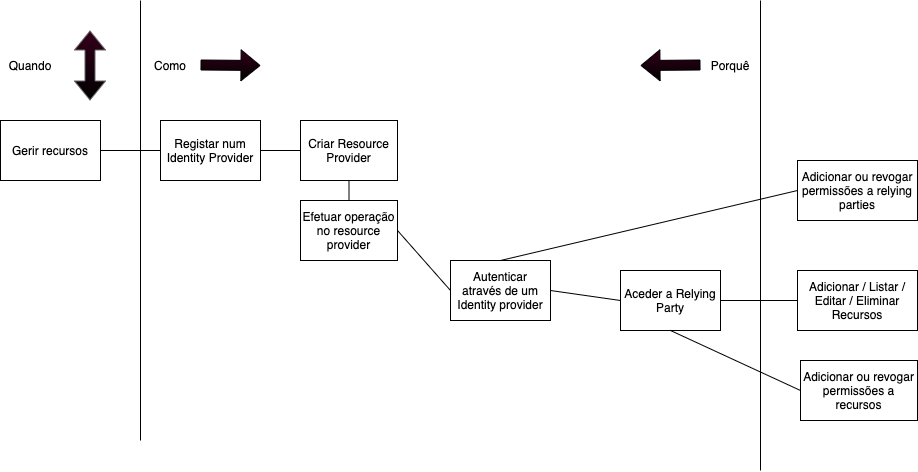
\includegraphics[width=1\textwidth]{figures/Canvas-FAST.png}
    \caption{Modelo Fast}
    \end{center}
\end{figure}

Este modelo permite perceber que o "core" de toda framework são os dados dos utilizadores. Essa é a grande falha do modelo actual de web, modelo este que torna a informação infinitamente redundante e a expropria do utilizador.
Um novo paradigma deve garantir que os dados estão sob alçada do seu utilizador, podendo o mesmo a qualquer momento tomar ações como revogar acesso a determinadas aplicações (\emph{relying parties} \footnote{POD ou aplicação cliente que utiliza um token providenciado por um servidor de identidade.}).

\section{Modelo Canvas}
\begin{figure}[h]
    \begin{center}
    % Requires \usepackage{graphicx}
    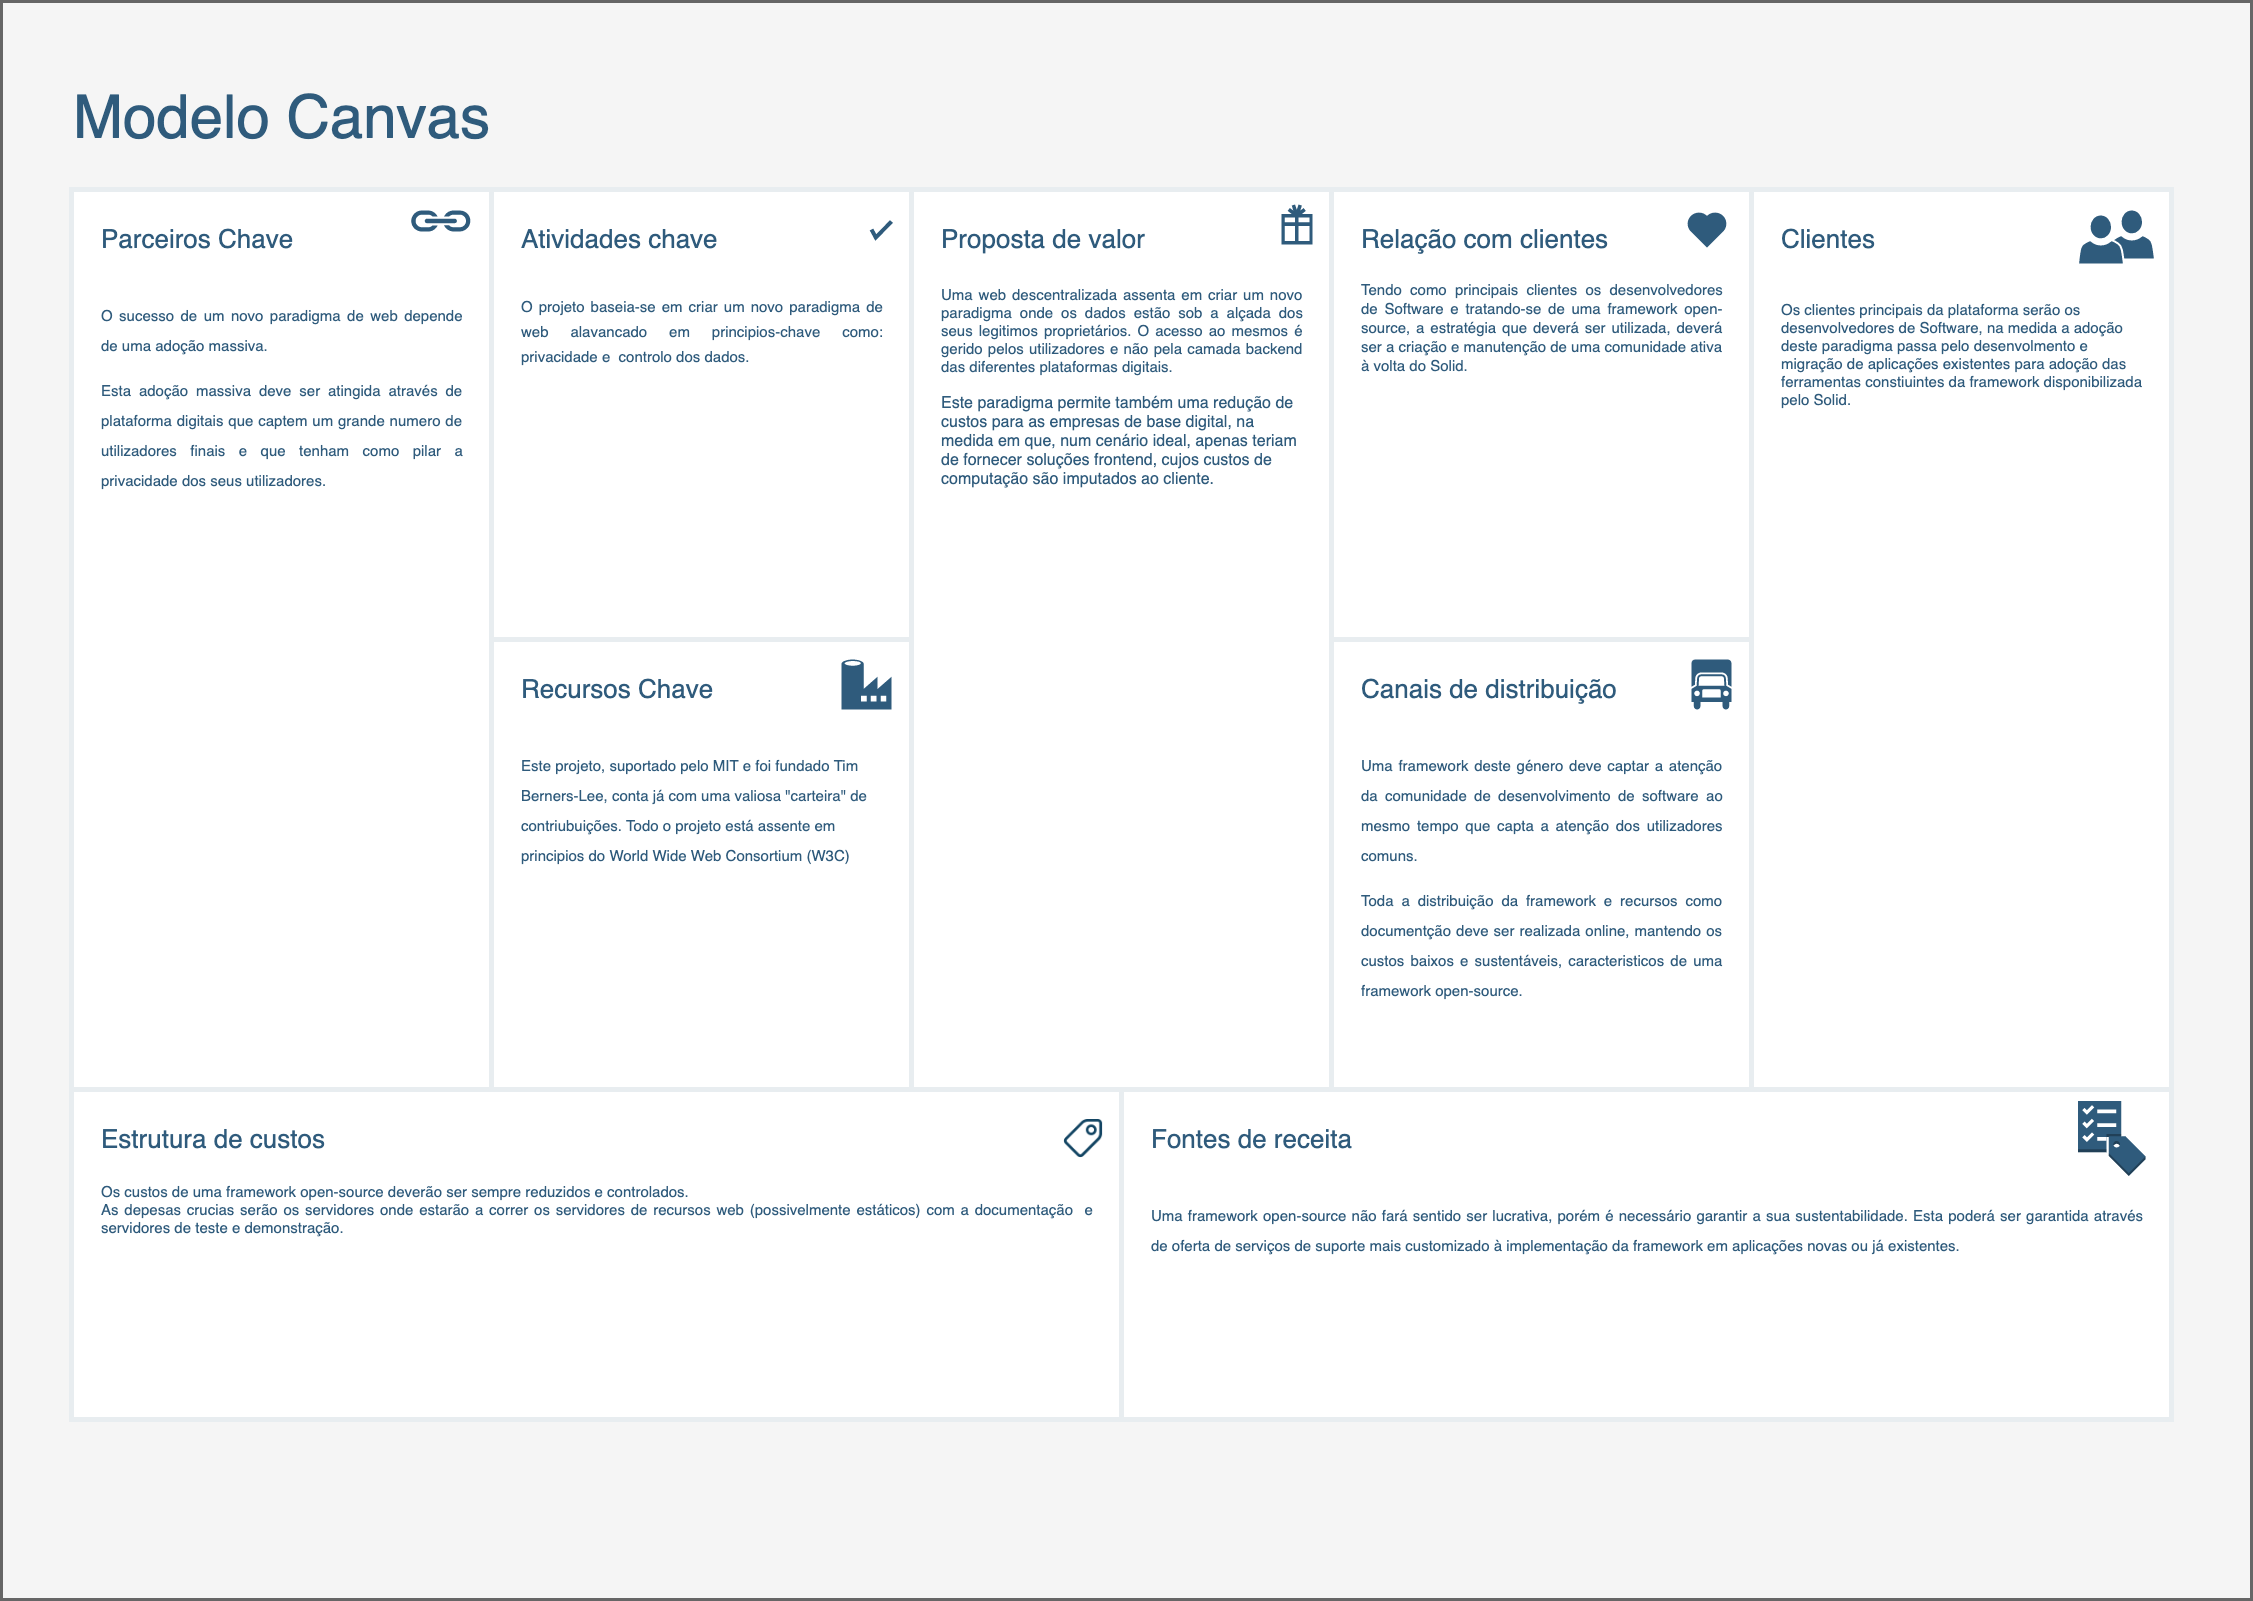
\includegraphics[width=1 \textwidth, angle=-90]{figures/Canvas-Canvas.png}
    \caption{Modelo Canvas}
    \end{center}
\end{figure}
